\section{Recurrent Models and Training Protocol}
\label{sec:recurrent}

\subsection{Recurrent networks and their gradients}
A recurrent network reads a window $x_1,\dots,x_T$ ($T=30$, $x_t\in\mathbb{R}^{14}$) and updates a hidden state
\begin{equation}
h_t=\tanh\!\left(W_x x_t+W_h h_{t-1}+b\right),
\end{equation}
where $W_x$ and $W_h$ are the input and recurrent weight matrices and $b$ is a bias.  The prediction is $\hat y=w^\top h_T+b_o$, with head weights $w$ and bias $b_o$.  Training by backpropagation through time (BPTT) unrolls the recurrence, and the gradient of the loss $\mathcal{L}$ with respect to an early state is
\begin{equation}
\frac{\partial \mathcal{L}}{\partial h_k}=\frac{\partial \mathcal{L}}{\partial h_T}\prod_{t=k+1}^{T}\frac{\partial h_t}{\partial h_{t-1}} .
\end{equation}
If the norm of each Jacobian factor is below one, the product shrinks geometrically with $T-k$ (vanishing gradients) and distant cycles stop influencing learning; if it is above one, the product grows (exploding gradients)~\cite{pascanu_2013_difficulty}.

\textbf{LSTM.}  The long short-term memory (LSTM) cell adds a cell state $c_t$ that is updated additively~\cite{hochreiter_1997_lstm,gers_2000_forget}:
\begin{align}
i_t&=\sigma(W_i[x_t,h_{t-1}]+b_i), & f_t&=\sigma(W_f[x_t,h_{t-1}]+b_f),\\
o_t&=\sigma(W_o[x_t,h_{t-1}]+b_o'), & g_t&=\tanh(W_g[x_t,h_{t-1}]+b_g),\\
c_t&=f_t\odot c_{t-1}+i_t\odot g_t, & h_t&=o_t\odot\tanh(c_t),
\end{align}
where $i_t$, $f_t$, $o_t$ are the input, forget and output gates, $g_t$ is the candidate update, $\sigma$ is the logistic function and $\odot$ is element-wise multiplication.  Because $\partial c_t/\partial c_{t-1}=f_t$ (a gate in $(0,1)$ rather than a repeated weight matrix), the gradient along the cell path is not forced to vanish.

\textbf{GRU.}  The gated recurrent unit (GRU) merges cell and hidden state and uses two gates~\cite{cho_2014_gru}:
\begin{align}
z_t&=\sigma(W_z[x_t,h_{t-1}]+b_z), & r_t&=\sigma(W_r[x_t,h_{t-1}]+b_r),\\
\tilde h_t&=\tanh(W_h[x_t,r_t\odot h_{t-1}]+b_h), & h_t&=(1-z_t)\odot h_{t-1}+z_t\odot\tilde h_t,
\end{align}
with update gate $z_t$ and reset gate $r_t$.  A GRU has three weight blocks per layer instead of four, hence fewer parameters.

\subsection{Training protocol}
The loss was the mean squared error on the scaled target,
$\mathcal{L}=\frac{1}{N}\sum_{n=1}^{N}\big(\hat y_n-y_n/100\big)^2$, with the true uncapped RUL $y_n$.  We used AdamW~\cite{loshchilov_2019_adamw}, whose update is
\begin{equation}
\theta\leftarrow\theta-\eta\left(\frac{\hat m}{\sqrt{\hat v}+\epsilon}+\lambda\theta\right),
\end{equation}
where $\theta$ are the weights, $\eta=10^{-3}$ the learning rate, $\hat m,\hat v$ the bias-corrected first and second moment estimates of the gradient, and $\lambda$ the weight decay.  The decay term is applied to the weights directly and is not passed through the adaptive scaling, which is what \emph{decoupled} means; with plain L2 regularization the penalty would be rescaled by $1/\sqrt{\hat v}$.  Dropout~\cite{srivastava_2014_dropout} multiplies the hidden vector by a Bernoulli mask, $\tilde h=m\odot h/(1-p)$ with $m_j\sim\mathrm{Bernoulli}(1-p)$, between recurrent layers and before the output layer.  Gradient clipping replaces a gradient $g$ by $g\cdot\min(1,\tau/\lVert g\rVert_2)$ with $\tau=1$~\cite{pascanu_2013_difficulty}.  Early stopping kept the weights of the epoch with the lowest mean absolute error over all windows of the 20 validation engines, with a maximum of 60 epochs and a patience of 8 epochs.  Because both the stopping epoch and the final configuration were chosen on these engines, the validation scores are slightly optimistic; the held-out test set is the unbiased check.  Training used the 80 training engines (16,390 windows) with batch size 256 and seed 42; windows of one engine overlap by 29 of 30 cycles, so the effective sample size is close to 80 rather than 16,390.

Each factor was varied alone around a baseline of two layers, 64 hidden units, dropout 0.2, weight decay $10^{-4}$ and patience 8, for both cell types.  A final configuration per model was chosen by the lowest validation-engine window MAE (differences below 0.05 cycles went to the smaller model), a rule fixed before the results were inspected; the 100 fixed validation points were not used for selection.

\subsection{Results}
Table~\ref{tab:reg} lists the validation-engine window MAE for every setting and Fig.~\ref{fig:sweeps} plots it together with the training MAE.  The selection rule chose a one-layer LSTM with 64 units and dropout 0.2 (20,545 parameters; \texttt{config\_lstm.json}) and a two-layer GRU with 64 units and dropout 0.3 (40,385 parameters; \texttt{config\_gru.json}).  Both used AdamW with weight decay $10^{-4}$.

Early stopping was the only regularizer with a clear effect.  Training for a fixed 60 epochs and keeping the last epoch raised the window MAE from 26.87 to 31.15 cycles (GRU) and from 28.42 to 31.95 (LSTM) while the training MAE fell to about 7 cycles.  Dropout and weight decay moved the score by at most 0.68 and 0.07 cycles, which is smaller than the seed-to-seed variation of a fixed configuration (26.78, 27.01, 27.20 for the GRU; 26.38, 27.17, 27.22 for the LSTM), so these effects cannot be separated from noise.  Weight decay is nearly inert because AdamW shrinks the weights by only $\eta\lambda=10^{-7}$ per step.  Gradient clipping was not needed to prevent divergence: the mean gradient norm per epoch peaked at 1.57 (GRU) and 1.31 (LSTM) with clipping at 1.0, and at 1.13 and 0.99 without it.

\begin{table}[t]
\centering
\caption{Validation-engine window MAE (cycles) for each one-factor change. Bold marks the baseline value. Single runs, seed 42.}
\label{tab:reg}
\footnotesize
\begin{tabular}{llcc}
\toprule
Factor & Value & GRU & LSTM\\
\midrule
Dropout & 0 & 26.95 & 28.68\\
 & 0.1 & 26.97 & 28.66\\
 & \textbf{0.2} & \textbf{26.87} & \textbf{28.42}\\
 & 0.3 & 26.78 & 28.01\\
 & 0.5 & 27.16 & 28.23\\
\midrule
Weight decay & 0 & 26.86 & 28.40\\
 & $10^{-5}$ & 26.86 & 28.40\\
 & \textbf{$10^{-4}$} & \textbf{26.87} & \textbf{28.42}\\
 & $10^{-3}$ & 26.80 & 28.44\\
\midrule
Patience & 3 & 27.39 & 28.50\\
 & \textbf{8} & \textbf{26.87} & \textbf{28.42}\\
 & 15 & 26.87 & 28.42\\
 & none (60 ep.) & 31.15 & 31.95\\
\midrule
Hidden units & 32 & 27.19 & 27.39\\
 & \textbf{64} & \textbf{26.87} & \textbf{28.42}\\
 & 128 & 27.77 & 27.06\\
\midrule
Layers & 1 & 27.01 & 26.38\\
 & \textbf{2} & \textbf{26.87} & \textbf{28.42}\\
 & 3 & 26.77 & 27.72\\
\bottomrule
\end{tabular}
\end{table}

\begin{figure*}[t]
\centering
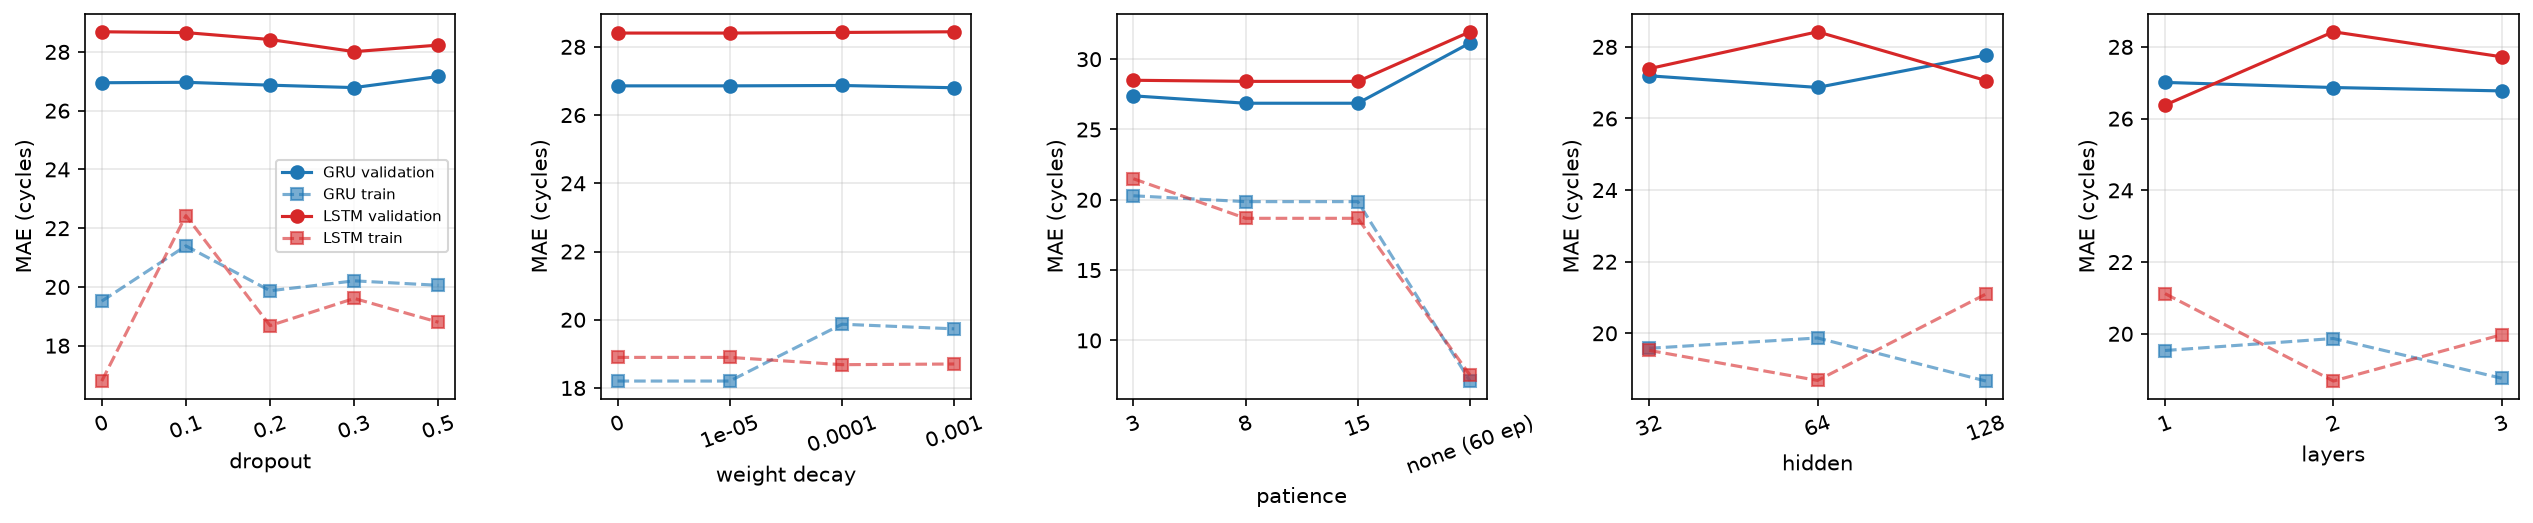
\includegraphics[width=\textwidth]{../results/phase2/figures/rnn_regularization_sweeps.png}
\caption{Validation-engine window MAE (solid) and training MAE in evaluation mode (dashed) against each setting; one run per point.}
\label{fig:sweeps}
\end{figure*}

Table~\ref{tab:final} gives the scores of the chosen models on the 100 fixed validation points.  The three-seed means of the LSTM and the GRU (20.14 and 22.98 MAE) are below the Random Forest value of Phase~1 (25.03), by 4.89 and 2.05 cycles, which is larger than the seed standard deviations; the RMSE falls from 40.17 to 33.18 (LSTM) and 36.61 (GRU).  The early-life MAE (true RUL above 125) remains high at 43.7 and 43.3 cycles for the saved models.  In the band above 200 cycles (five points) the mean error is $-124.7$ (LSTM) and $-115.8$ (GRU) cycles, so the underprediction of Phase~1 is not removed; five points are too few for a firm conclusion.  At the matched two-layer, 64-unit setting the LSTM has 53,825 parameters against 40,385 for the GRU and needs 1.48 s per epoch against 1.14 s on one CPU thread.  The seed 42 baselines of the two cell types differ by one cycle of MAE (21.83 and 22.83), within seed noise, so the evidence for one cell type is weak.

\begin{table}[t]
\centering
\caption{Chosen models on the 100 validation points. Mean $\pm$ standard deviation over seeds 42, 43, 44; early and late MAE are for the saved seed 42 model. The Random Forest row is the Phase~1 result.}
\label{tab:final}
\footnotesize
\begin{tabular}{lcccc}
\toprule
Model & MAE & RMSE & Early MAE & Late MAE\\
\midrule
LSTM (1 layer, 64) & $20.14\pm1.46$ & $33.18\pm2.46$ & 43.73 & 12.55\\
GRU (2 layers, 64) & $22.98\pm0.49$ & $36.61\pm0.90$ & 43.34 & 17.49\\
Random Forest (Phase 1) & 25.03 & 40.17 & 49.33 & 18.17\\
\bottomrule
\end{tabular}
\end{table}

\begin{figure}[t]
\centering
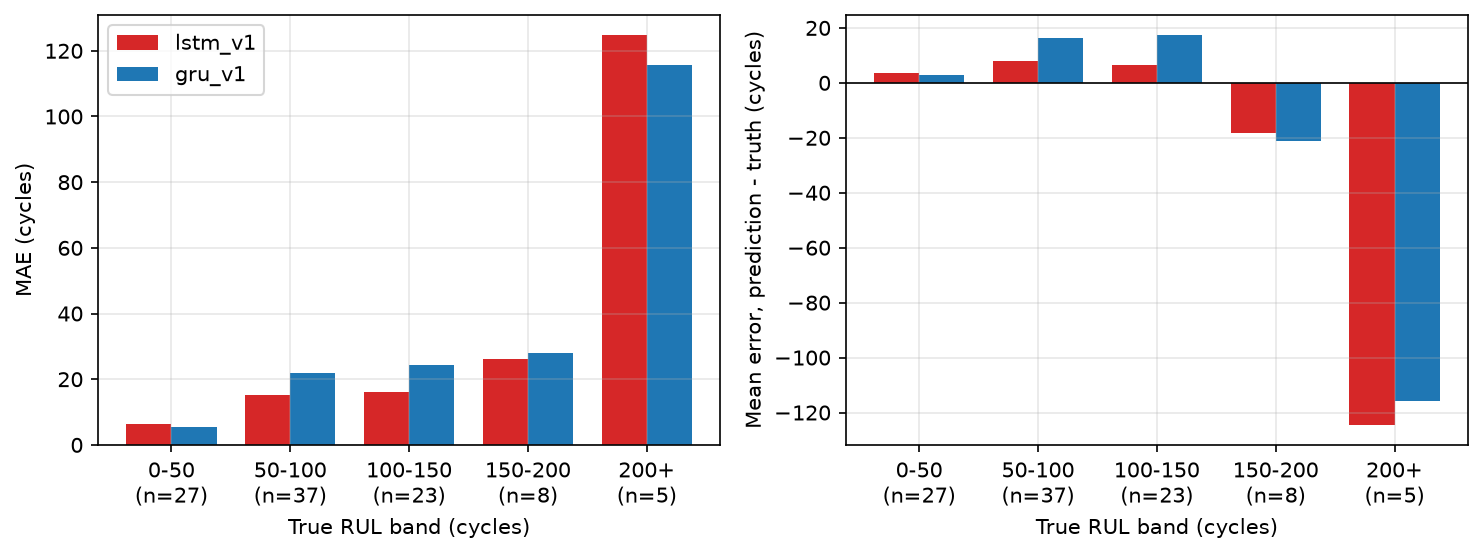
\includegraphics[width=\columnwidth]{../results/phase2/figures/rnn_error_by_band.png}
\caption{Error by true-RUL band for the saved models, with the number of validation points per band.}
\label{fig:bands}
\end{figure}
